%Carattere dimensione 12
\documentclass[12pt]{report}

%Margini e interlinea
\usepackage[top=1in, bottom=1in, left=1.2in, right=1in]{geometry}
\pagestyle{plain}
\linespread{1.5}

%Librerie utili
\usepackage[english]{babel}
\usepackage[utf8]{inputenc}
\usepackage{adjustbox}
\usepackage{libertine}
\usepackage{graphicx}
\usepackage{floatflt}
\usepackage{blindtext}
\usepackage{enumitem}
\usepackage{amsthm}
\usepackage{listings}
\usepackage{listingsutf8}
\usepackage{amsmath}
\usepackage{amssymb}
\usepackage{bbold}
\usepackage{framed}
\usepackage{minibox}
\usepackage{float}
\usepackage{wrapfig}
\usepackage{longtable}
\usepackage[strict]{changepage}
\usepackage{pgfplots}
\usepackage{tikz}
\usepackage{xcolor}
\usepackage{braket}
\usepackage{refstyle}
\usepackage{booktabs}  % For better table rules
\usepackage{caption}   % For custom captions
\usepackage{subcaption}
\usetikzlibrary{matrix}
\pgfplotsset{width=11cm,compat=1.9}
\usepgfplotslibrary{external}
\tikzexternalize

\begin{document}

\begin{titlepage}

\begin{center}
	\textbf{ Dipartimento di Fisica\\ Corso di Laurea Magistrale in Fisica\\}
	\vspace{15mm}
    {\LARGE{\bf First Results of Closure Tests}}\\
	\vspace{3mm}
	\end{center}

\vspace{36mm}

\begin{minipage}[t]{0.47\textwidth}

	{\large{\bf Presented by: \\ Kamil Laurent\\ }}
\end{minipage}

\vspace{18mm}

\end{titlepage}

\tableofcontents

\chapter{Closure Testing}
\section{L0 distributions}
At L0 we test wether the mimimiser used by our fitting procedure is able to find the real minimum of the Error Function (in this case the $\chi^2$) in the parameters space. In particular we consider two parametrization used in the past by the MAP collaboration: MAP22g2 \cite{MAP22}  and PV19x \cite{MAP19}. 

We first genarated two set of pseudo-data L0 using the MAP22g52 and the PV19x parametrizations as imput for the constructions of the TMD PDFs and FFs; both at N3LL accuracy. The parametrization MAP22g52 can reconstruct both PDFs and FFs, so we were able to generate the full dataset including SIDIS and DY phisical observables. In the case of PV19x, the parametrization is only able to describe the TMD PDFs, so from this set of parameters we only generated the Drell-Yan cross sections and we exluded all the SIDIS experiments. In this second case, the dataset is much smaller than in the first case. In Table~\ref{tab:MAP22_real} and ~\ref{tab:PV19_real} one can see the parameters used for generating the "real" distributions in the two cases (i.e. the pseudo-data at L0). 

\begin{table}[h]
    \caption{Parametrization: \textbf{MAP22g52}}
    \label{tab:MAP22_real}
    \centering
   \begin{tabular}{|c|c|}
    \hline
    \textbf{parameter} & \textbf{value}\\
    \hline
    $g_2$ & 0.2486239 \\
    $N_1$ & 0.31811409 \\
    $\alpha_1$ & 1.1539107 \\
    $\sigma_1$ & 0.51913972 \\
    $\lambda$ & 1.7426787 \\
    $N_3$ & 0.0043346176 \\ 
    $\beta_1$ & 10.845024 \\ 
    $\delta_1$ & 0.0071260428 \\
    $\gamma_1$ & 1.5329148 \\
    $\lambda_F$ & 0.062387441 \\ 
    $N_{3B}$ & 0.21741506 \\
    $N_{1B}$ & 0.12914044 \\ 
    $N_{1C}$ & 0.015972667 \\
    $\lambda_2$ & 0.020872149 \\
    $\alpha_2$ & 4.2745401 \\
    $\alpha_3$ & 4.3751368 \\ 
    $\sigma_2$ & 0.41386142 \\ 
    $\sigma_3$ & 12.625959 \\ 
    $\beta_2$ & 4.2674647 \\
    $\delta_2$ & 0.16113037 \\
    $\gamma_2$ & -0.0026776056\\
    \hline
\end{tabular}
\end{table}

\begin{table}[h]
    \caption{Parametrization: \textbf{PV19x}}
    \label{tab:PV19_real}
    \centering
   \begin{tabular}{|c|c|}
    \hline
    \textbf{parameter} & \textbf{value}\\
    \hline
    $g_2$ & 0.037923106 \\
    $N_1$ & 0.51881393 \\ 
    $\alpha$ & 0.20314198 \\
    $\sigma$ & 0.37327219 \\ 
    $\lambda$ & 0.57973261 \\
    $N_{1B}$ & 0.039554376 \\ 
    $\alpha_B$ & 0.067696657 \\ 
    $\sigma_B$ & 0.36307837 \\ 
    $g_{2B}$ & 0.011221607 \\
    \hline
\end{tabular}
\end{table}

\chapter{Results}

In this chapter we present the results of various closure tests on several fitting procedures. As mentioned before the closure testing involves different levels that test different type of errors. Here we present the result of the closure testing at level 0 (L0: pseudo-data without fluctuations), level 1 (L1: pseudo-data fluctuated using multivariate gaussian distributions) and level 2 (L2: a set of Monte Carlo replicas of the pseud-data L1).

\section{Choice of the Minimiser}

With the level 0 datasets we first tested the minimisers used by the software Nanga Parbat (Cerer and Minuit). For this test we made 100 fits of the replica 0 of the pseudo-data generated by the MAP22g52 parametrization. We name this test g52oMAP22 (g52 parametrization used over data generated with MAP22 parametrization). For each one of this 100 fits, we start the minimization in a different point in the parametrs space. We made this test using Ceres and Minuit.
This test is made to know if the minimizer is able to find the correct minimum starting from a casual point or if the found minimum is dependent from the starting point of the minimizer. Using the $\chi^2$ as a metric for the accuracy of the fit, we obtain a very good result when we use Ceres as a minimizer: in the majority of the cases the minimizer stops at a $\chi^2 \sim \mathcal{O}(10^{-14})$ only in $10\%$ of the cases the minimizer didn't reach that accuracy. In the other hand, when we use Minuit as minimizer, we found in the best cases $\chi^2 \sim \mathcal{O}(10^{-4})$. We repeated the same test using the PV19 parametrization over a dataset generated from PV19 (PV19oPV19) and we obtained similar results. We made an ulterior test using the MAP22g52 parametrization over a dataset generated from PV19 (g52oPV19), using both Ceres and Minuit. The results of the Ceres-Minuit comparison are shown in Table~\ref{tab:CeresVsMinuit}. From these results is clear that Ceres does a better job. From now on we continue our closure tests using Ceres as the only minimizer and we leave Minuit apart. 

\begin{table}[h]
    \caption{Ceres-Minuit comparison}
    \label{tab:CeresVsMinuit}
    \centering
   \begin{tabular}{|c|c|c|}
    \hline
    \textbf{Test} & \textbf{Minimiser} & $\chi^2$ \\
    \hline
    g52oMAP22 & Ceres & $\mathcal{O}(10^{-14})$ \\
    g52oMAP22 & Minuit & $\mathcal{O}(10^{-4})$ \\
    PV19oPV19 & Ceres & $\mathcal{O}(10^{-13})$ \\
    PV19oPV19 & Minuit & $\mathcal{O}(10^{-5})$ \\
    g52oPV19 & Ceres & $\mathcal{O}(10^{-1})$ \\
    g52oPV19 & Minuit & not convergent \\
    \hline
\end{tabular}
\end{table}

\section{L0 Results}

We already mentioned that a closure test of the MAP22g52 parametrization over a dataset generated by the same parametrization (g52oMAP22) closes with a $\chi^2\sim \mathcal{O}(10^{-14})$. Similarly, the PV19oPV19 tes closes with  $\chi^2\sim \mathcal{O}(10^{-14})$. Both g52oMAP22 and PV19oPV19 are tests of the fitting procedure in which we assume to know the \textit{real} law (the real functional form of the TMD PDFs and FFs) and we assume that we only have to fix the parameters. In other words we are assuming that our parametrization maches completly the real law of nature, and we have to find the free parameters by executing a fit. This first results demonstrates that in this particular case our fitting procedure is well constructed ad is able to find the real parameters with a very high precision.

However, the most likely situation is that we don't know the real functional form of the TMD PDFs and FFs, and our parametrization is at best a good approximation of the real law. We now want to answer to this question: if the real law is different from our parametrization, the minimizer is still able to find a functional form that matches the real TMDs? 

To answer to this question we made two different closure test al L0 in which the parametrization of the real distribution is different from the parametrization used in the fit: g52oPV19 and PV19oMAP22.

\subsection{L0 g52oPV19}
In this first case we have a dataset generated with the PV19 TMD PDF and we fit this dataset using the MAP22g52 parametrisation. This is the case in which our parametrization is more complex than the real form of the TMD, and we want to kow if our fitting procedure is able to reproduce the real (simpler) law. 

Also in this case we produced 100 fits of the replica 0 starting each time from a different point in the parameter space. We obtained from this fitting procedure 89 convergent fits, with a mean $\chi ^ 2$ of $\chi^2_{mean} = 0.1462$.

From a first look we should conlude that this test does not close, but if we take a closer look to the non perturbative TMD functional  forms (the $f_{NP}(x, b_T, \zeta)$) given by the fit, we clearly see that there are two class of functions (figure \ref{fig:f1}). Plotting the real and the predicted $f_{NP}(x, b_T, \zeta)$, one can add a condition on the Mean Squared Distance between the two distribution, defined as:

\begin{equation}
    MSD = \frac{\sum_{i=1}^{N_{points}}(f_{NP}^{real} - f_{NP}^{pred})^2}{N_{points}} \label{eq:msd}
\end{equation}

where the real and predicted $f_{NP}(x, b_T, \zeta)$ are plotted in $x = 0.1$, $\zeta = Q^2 = 100$ and $b_T \in [0, 10]$. $N_{points}$ is the number of points used in the $b_T$ interval to plot the distributions.

Using this condition we obtain 47 fits where $MSD <= 0.0015$ (figure \ref{fig:f2}). \\

We conclude that the minimiser finds a minimum that is dependent from the starting point in the paramters space. There are two distinct minimum, one corresponding to the real distribution and one leading to an incorrect prediction of the TMD PDF. The minimiser that we use (ceres) finds the correct minimum in roughly half of the cases. This leads to a $\chi^2_{mean} = 0.146$, but this $\chi^2_{mean}$ is given by a class of acceptable resuts (with $\chi^2$ arount $0.05$) and a class of incorrect results (with $\chi^2$ arount $0.25$). In figure \ref{fig:chi2_dist_1} one can clearly see that the $\chi^2$ is divided into two class. If we only consider the best fits (the acceptable results) and we throw away the replicas that converge but have a $\chi^2 > 0.07$, the result of the closure test would be much better. Anyway, if we take the $\chi^2$ of the first tests (where we use the same paramterization for the fit and the generation of pseudo-data) as a treshold, even in the best fits the L0 g52oPV19 test does not close. 

\begin{figure}[!hbp]
    \begin{subfigure}[b]{0.5\textwidth}
        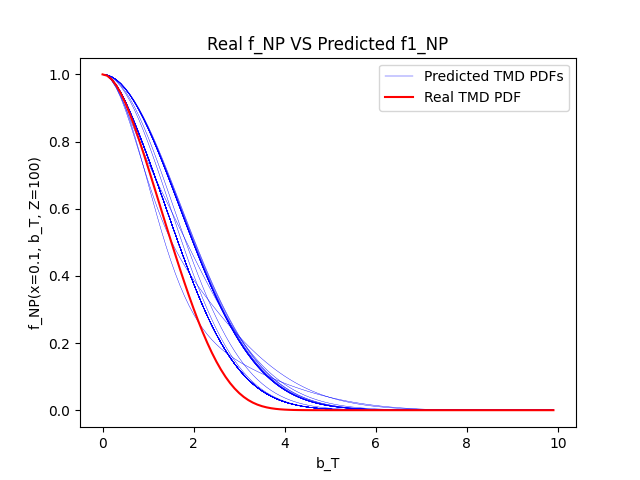
\includegraphics[width=\textwidth]{Images/L0_tests/Convergent_Dist_0.01_Q_10.png}
        \caption{All Predicted TMDs}
        \label{fig:f1}
    \end{subfigure}
    \hfill
    \begin{subfigure}[b]{0.5\textwidth}
        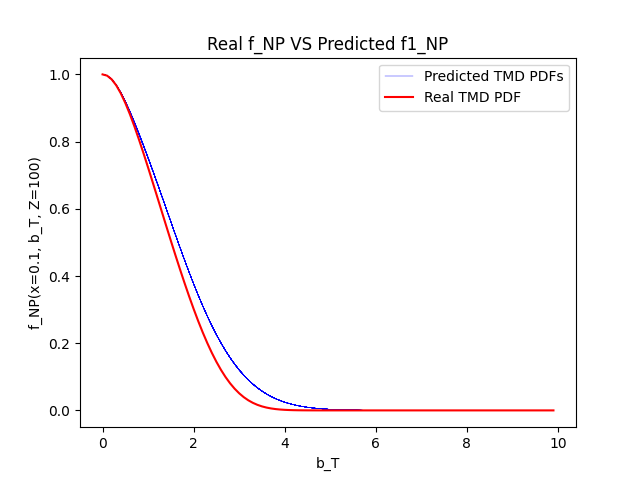
\includegraphics[width=\textwidth]{Images/L0_tests/Convergent_Dist_0.0015_Q_10.png}
        \caption{Predicted TMDs with $MSD < 0.0015$}
        \label{fig:f2}
    \end{subfigure}
    \caption{Real Vs $f_{NP}(x=0.1, b_T, \zeta=100)$ in L0 g52oPV19}
\end{figure}

\begin{figure}[!h]
    \centering
    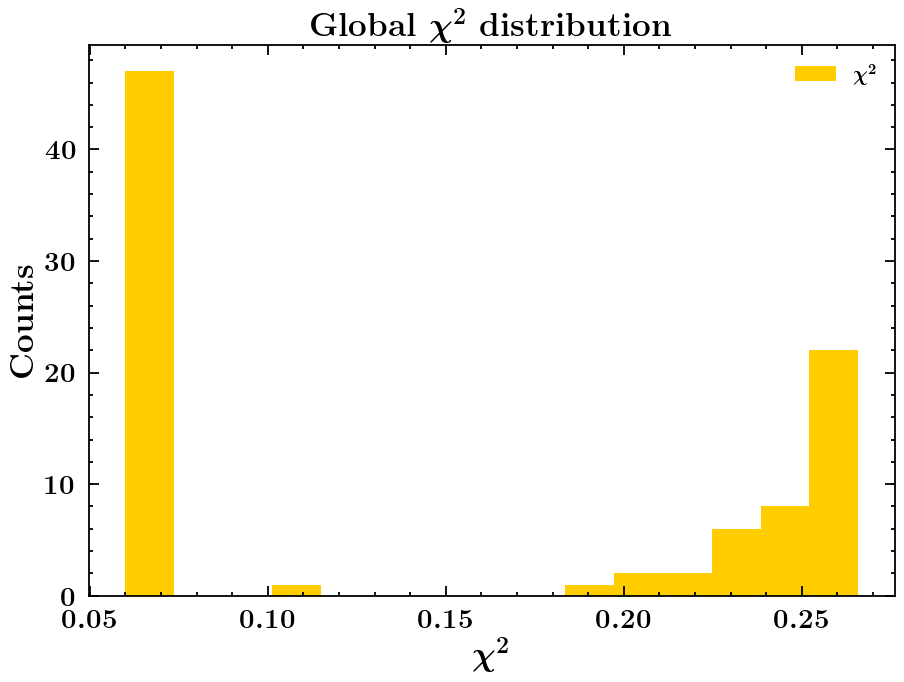
\includegraphics[scale=0.5]{Images/L0_tests/Globalchi2_g52oPV19.png}
    \caption{$\chi^2$ distribution in L0 g52oPV19}
    \label{fig:chi2_dist_1}
\end{figure}

\subsection{L0 PV19oMAP22}

We make now the opposite exercise with respect to the previous section. With the PV19oMAP22 test at L0 we execute 100 fits using the PV19 parametrization over a dataset generated from the MAP22g52 parametrization. For each fit we start from a different point in the parameter space. Also in this case we only use the Drell-Yan experiments, because the PV19 parametrization does not take into account the TMD FFs used to describe the SIDIS processes.

The PV19 non perturbative function is simpler than the MAP22g52 $f_{NP}(x, b_T, \zeta)$ (that we assume to be the real distrbution). Therefore, we expect to obtain worse results than those of the g52oPV19 test, because we are searching to capture a complex functional form (MAP22) with a simpler one (PV19).\\

Surprisingly the test leaded to better results than before. The minimiser found in $100\%$ of the replicas the same minimum and we get a $\chi^2_{mean} = 0.017$, that is one order of magnitude smaller than in the previuos test. We can see from the $\chi^2$ distribution (figure \ref{fig:chi2_dist_2}) that in this case the minimiser fall in the right minimum independently from the starting point in the parameter space. The $\chi^2$ is computed on the predictions of the experimental cross sections, but in this artificial case we know exactly the real distribution that we are searching. We can ask ourselfes if the predicted $f_{NP}(x, b_T, \zeta)$ matches the real non perturbative function, so as we done before we compute the $MSD$ (eq \ref{eq:msd}) for this test, and we find out that the condition used before ($MSD <= 0.0015$) is respected in 100\% of the fits. Going further we can divide by $10$ the $MSD$ treshold and we still get $MSD <= 0.00015$ in 100\% of the replicas (figure \ref{fig:MSE_PV10oMAP22}).   

\begin{figure}[!h]
    \centering
    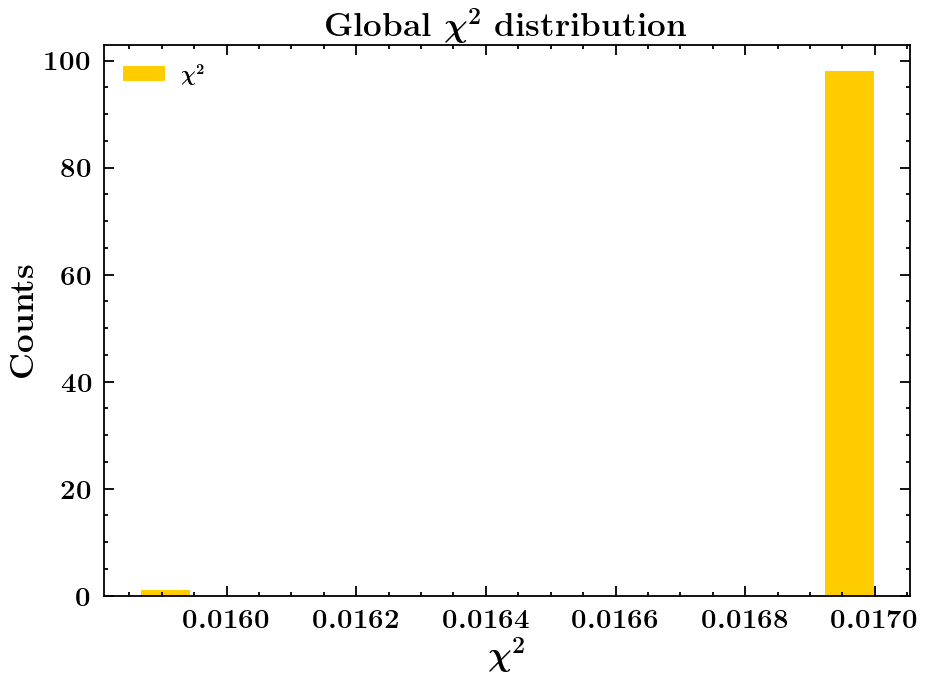
\includegraphics[scale=0.5]{Images/L0_tests/Globalchi2_PV19oMAP22.png}
    \caption{$\chi^2$ distribution in L0 PV19oMAP22}
    \label{fig:chi2_dist_2}
\end{figure}

\begin{figure}[!h]
    \centering
    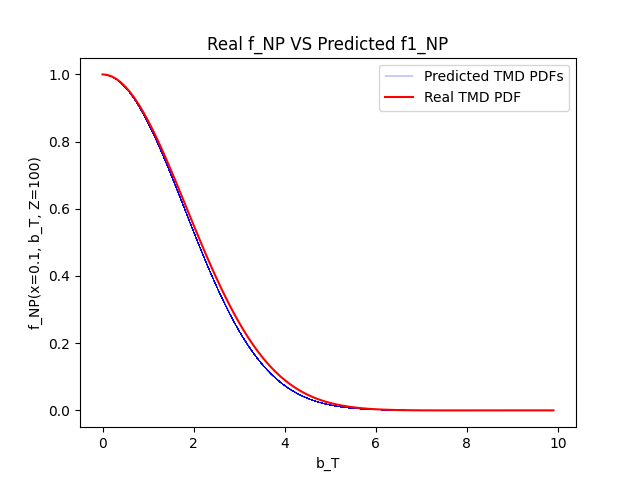
\includegraphics[scale=0.8]{Images/L0_tests/real_vs_predictions0.00015_Q_10.png}
    \caption{Real Vs Predicted $f_{NP}(x=0.1, b_T, \zeta=100)$ in L0 PV19oMAP22}
    \label{fig:MSE_PV10oMAP22}
\end{figure}

There are many possible reasons why the PV19oMAP22 test leads to better results than the g52oPV19 test. We identified two main reasons (that are to be tested).

The first reason is a limit of the minimiser. In particular, using a more complex parameters space (that of the MAP22g52 parametrization), Ceres cannot distinguish the true minimum from a local one, and is able to find the correct minumum only in roughly 50\% of the cases. When we simplify the parameter space (i.e. with the PV19x parametrization), Ceres has no doubt on what minimum to choose and finds the correct parameters configuration in 100\% of the cases. This is a limit of the minimiser, and we cannot do much to solve this problem, since we cannot modify the minimiser. However, in the test g52oPV19 we find a worst result compared to the PV19oMAP22 test even in the cases in which the minimiser fall in the correct minimum. This suggest that there could be some room of improvement also in the parametrization itself. Therefore, the other reason why PV19oMAP22 leads to better results than g52oPV19 could be that the PV19 parametrization was written without taking into account the SIDIS observables and is very accurate in describing the fenomenology of Drell-Yan experiments. It is possible that the MAP22 parametrization sacrifice some accuracy in describing Drell-Yan cross sections in order to include the SIDIS phenomenology within the domain of a single TMD PDF. According to the theory, we should have the same non perturbative functions that describes both DY and SIDIS phenomenology. Therefore, the search of a global $f_{NP}(x, b_T, \zeta)$ justifies a minor loss of accuracy in describing DY data. This loss of accuracy is amplified by our test conditions in which we used only Drell Yan data for the fits. \\

To test this hypotesis we should try to generate the SIDIS L0 dataset using the PV19 parametrization for the TMD PDF and an external TMD Fragmentation Function (FF), then repeat the g52oPV19 test to see the behaviour of the minimiser with the full dataset.\\

Here we leave a table with the results reached so far:

\begin{table}[h]
    \caption{L0 results}
    \label{tab:L0_results}
    \centering
    \begin{adjustbox}{width=\textwidth}
        \begin{tabular}{|c|c|c|c|c|c|}
        \hline
        \textbf{name} & \textbf{fit parametrizetion:} & \textbf{pseudo-data  generated with:} & \textbf{mean $\chi^2$} & \textbf{best $MSD$} & \textbf{closure}\\
        \hline
        g52oMAP22 & MAP22g52 & MAP22g52 & $\mathcal{O}(10^{-14})$ & / & yes \\
        PV19oPV19 & PV19x & PV19x & $\mathcal{O}(10^{-13})$ & / & yes \\
        g52oPV19 & MAP22g52 &  PV19x & 0.146 & $< 0.0015$ & no \\
        PV19oMAP22 & PV19x & MAP22g52 & 0.017 & $< 0.00015$& no \\
        \hline
    \end{tabular}
\end{adjustbox}
\end{table}


\end{document}


\bibliography{references}
\bibliographystyle{plain}

\end{document}